\documentclass[10pt]{article}

%---------------------------------------------------------------------

\usepackage[a4paper, headsep=0in,bindingoffset=0in,%
left=0.9in,right=0.9in,top=0.9in,bottom=0.9in,%
footskip=.25in]{geometry}


\usepackage[english]{babel}   
\usepackage[utf8]{inputenc}  
\usepackage{sectsty}
\usepackage{subcaption}
\usepackage{wrapfig}

\usepackage{lineno}
\linenumbers
\usepackage{graphicx}
\usepackage[
backend=bibtex,
style=numeric,
sorting=none
]{biblatex}
\addbibresource{feb25bib.bib}
\usepackage{amsfonts}
\graphicspath{{/Users/emilyolafson/GIT/stroke-graph-matching/apaper/figs/}}

\renewcommand{\baselinestretch}{1.3}
\usepackage{verbatim}
\usepackage{listings}
\usepackage{indentfirst}
\setlength{\parindent}{1cm}
%\setlength{\parskip}{0.5cm}

\setlength{\headsep}{1pt}
%---------------------------------------------------------------------

\begin{document} 
	\sectionfont{\large}
	\title{Functional connectome reorganization after pontine stroke is associated with better motor  	outcomes}
	\maketitle
 	\author{Emily Olafson, Keith Jamison, Hesheng Liu, Danhong Wang, Joel Bruss, Aaron Boes, Amy Kuceyeski}%, Keith Jamison, PhD\inst{1}, Hesheng Liu, MD\inst{2}, Danhong Wang, MD\inst{2},Joel Bruss, PhD\inst{3}, Aaron Boes, MD PhD\inst{3}, Amy Kuceyeski, PhD\inst{1}}
	% E-MAILS
	%\address{Weill Cornell Medical College, \inst{2} Harvard Medical School, \\ \inst{3}Massachusetts General Hospital, \inst{4}University of Iowa 
	%}
	
	%---------------------------------------------------------------------
	\section*{Introduction}
	Motor deficits are the most common and disruptive symptoms of ischemic stroke. Spontaneous recovery of motor function occurs for most patients \cite{Duncan2000-uj}, and is dependent on the ability of brain networks to functionally reorganize and compensate for lost function \cite{Corbetta2005-ra}. As demonstrated by animal models, the functionality of damaged motor regions may be adopted by surviving tissue around the lesion, but brain areas distant to the lesion with similar function and connectivity as the damaged area have also been shown to compensate in animals, typically when the initial infarct is large \cite{Winship2009-af, Adam2020-jk, Murata2015-ss, Brown2009-jn}.
	\\
	
	In humans, functional reorganization underlying post-stroke motor recovery has been studied with resting-state functional magnetic resonance imaging (fMRI). Strong evidence suggests that crucial to eventual motor recovery is the restoration of interhemispheric resting-state functional connectivity (FC) between the primary motor cortices \cite{Carter2010-er, Urbin2014-iq, Rehme2013-ap}, but less is known about how functional networks change on a greater spatial and temporal scale after stroke. Altered network topology \cite{Wang2010-or} and recruitment of other networks aside from the motor network such as the frontoparietal network \cite{Hordacre2021-ct, Pool2018-px} have been implicated in the recovery process, but network changes at a high temporal resolution have not been well documented.
	\\
	
	Prior studies investigating neural correlates of motor recovery have focused almost exclusively on supratentorial strokes that impact the internal capsule and surrounding areas.  Infratentorial pontine strokes, which impact the connections between motor cortex and the cerebellum \cite{Lu2011-ow}, and account for roughly 7 percent of all ischemic strokes \cite{Saia2009-ik}, may have different sources of motor deficits and mechanisms of recovery-related reorganization from those of supratentorial strokes. Reduced blood flow measured by arterial spin labeling has been observed in the cerebellum and cortical regions in pontine stroke \cite{Wei2020-gj, Wang2019-jr} and longitudinally, changes in cerebral blood flow in cortical areas including the supramarginal gyrus and middle occipital gyrus were related to motor recovery.  Areas with abnormal blood flow over time also had abnormal FC \cite{Wei2020-gj}, and increased degree centrality in the ipsilesional cerebellum has been related to better motor recovery \cite{Liu2019-mj}. The network changes associated with functional damage and subsequent recovery in pontine stroke have yet to be assessed in a longitudinal study.
	\\
	
	Another key element of stroke recovery is diaschisis, a process by which remote brain areas anatomically connected to the lesion undergo structural and functional changes \cite{Carrera2014-ah}. Functional impairment and subsequent reorganization of areas anatomically connected to the lesion may be an important component of the recovery process that is still being explored. In this study, we propose a novel measure to capture adaptive functional plasticity after pontine stroke, outlined below, and connect it to patterns of structural disruption after stroke. 
	\\
	
	Connectivity to the rest of the brain is one aspect of a brain region's functional role in the network. We propose that instances of functional reorganization over time, as in the case of adjacent surviving tissue adopting the functional role of lost tissue, may be captured by identifying brain regions whose pattern of FC with the rest of the brain is more closely matched by a different brain region at a later date. Considering functional connectomes as graph, the task of identifying similar nodes (gray matter regions, in this case) between two functional connectomes can be considered a graph matching problem \cite{Conte2004-ro}. Graph matching has been applied recently to map individual structural connectomes to their functional connectomes \cite{Osmanlioglu2019-ao}. Conceptually, the process of graph matching exchanges the labels of nodes when doing so results increased similarity of the two networks. When two regions exchange FC profiles, the regions are said to have been ‘remapped’. We hypothesize that brain regions with more structural damage due to the lesion will more frequently functionally reorganize; that more impaired subjects will have more global functional reorganization; and that the amount of functional reorganization will correlate with the change in motor impairment between subsequent sessions.
	

	\section*{Methods} \label{sec:firstpage}
	
	\subsubsection*{Data description}
	 Twenty-three first-episode stroke patients (34-74 years old; mean age 57 years; 8 female) with isolate pontine infarcts. 15 subjects had right brainstem infarcts, 9 had left brainstem infarcts (Figure \ref{lesioncount}), and is described previously  \cite{Lu2011-ow}. Patients were scanned five times during a period of 6 months - 7, 14, 30, 90 and 180 days after stroke onset (Figure \ref{FMscores}) on a 3T TimTrio Siemens using a 12-channel phase-array head coil. Structural images were acquired using a sagittal MP-RAGE three-dimensional T1-weighed sequence (TR, 1600ms; TE 2.15ms; flip angle, 9°, 1.0 mm isotropic voxels (FOV, 256 x 256). Each MRI session involved two to four runs (360s each run) of resting-state fMRI. Subjects were instructed to stay awake and keep their eyes open; no other task instruction was provided. Images were acquired using the gradient-echo echo-planar pulse sequence (TR, 3000ms; TE, 30ms; flip angle, 90°, 3 mm isotropic voxels).
	\begin{figure}[h]
	   	\begin{center}
			\includegraphics[width=0.6\textwidth]{lesioncount.png}
			\caption{Distribution of lesions across the brain. Colors indicate the number of subjects with a lesion in that location.}
			\centering
			\label{lesioncount}
		\end{center}
	\end{figure}

	\begin{figure}[h]
	\begin{center}
		\includegraphics[width=0.6\textwidth]{FM_overtime.png}
		\caption{Fugl-Meyer scores for all subjects over sessions. Note that for subjects 6, 12, 20, 22, and 23 scores are missing. For subjects 6, 12, and 20, functional data is also missing}
		\centering
		\label{FMscores}
	\end{center}
\end{figure}

	\subsubsection*{Structural data processing}
	Preprocessing of the longitudinal structural data included registration of each subject’s session 2-5 T1 scans to the space of session 1, collapsing co-registered files to an average, creation of a skull-stripped brain mask, followed by manual editing and binarization of the hand-edited mask. Each mask was then pushed to each of the session 2-5 T1s in native space using the inverse registration acquired from the first step. This was followed by bias field correction of the 5 T1 scans, transformation of native-space bias field-corrected data back to session 1 space, and the creation of an average bias field-corrected scan for each subject. Lesion masks were hand-drawn on these transformed T1 scans by ADB and JEB.
	
	\subsubsection*{Functional data processing}
	Preprocessing of the longitudinal functional data was performed using the CONN toolbox, including functional realignment of volumes to the first volume, slice timing correction, segmentation and normalization, smoothing with a 4mm FWHM kernel, followed by a denoising protocol (CompCor \cite{Behzadi2007-zt}) which regressed out the CSF and WM signal,as well as realignment parameters. Temporal band pass filtering (0.008 - 0.09Hz),motion correction, despiking and global signal removal regression were also performed.  Regional time series data was acquired by parcellating the scans into 268 non-overlapping brain regions using a functional atlas defined for healthy controls \cite{Shen2013-zn} and averaging the time course of all voxels with a region.  Several analyses involve further parcellating of the 268-node atlas into 8 subnetworks \cite{Finn2015-er} (Figure \ref{networks}).
	
	
	\subsubsection*{Functional connectivity calculation}
	 Functional connectivity (FC) matrices were calculated as the regularized inverse of precision matrices. Calculating FC using precision minimizes the effect of indirect connections and has been shown to result in FC that are more similar to structural connectivity \cite{Wodeyar2020-kz, Liegeois2020-ua}. To compute the precision FC, we first took the unregularized inverse of the correlation matrix for each subject and averaged them over the sample to obtain the population-level precision matrix. We then calculated the individual’s precision matrices using Tikhonov regularization, which adds a positive term to the diagonal of the precision matrix before inversion where I is the identity matrix and $ \lambda $ is the regularization parameter. Gamma $\gamma \in [0,1]$ was chosen via a grid search to be the value that minimized the root mean squared error of the Frobenius norms between the regularized subject precision matrices and the population-level unregularized precision matrix, and was found to be $\gamma = 0.58$ (Supplementary Fig \ref{precision}).
	
	\subsubsection*{Estimated structural disconnection}
	Deficits from subcortical stroke may be related to damage at distant sites via metabolic diaschisis \cite{Hillis2002-dz, Corbetta2015-ez}. In order to account for the impact of lesions on the structural connectome, the extent of regional structural (white matter) connectivity disruption due to the lesion was assessed for each stroke subject with the Network Modification (NeMo) Tool \cite{Kuceyeski2013-nk}. The Network Modification (NeMo) Tool v2 requires only an individual’s lesion mask in MNI space, which was obtained as described above, to produce an estimate structural disconnection for each brain region. The newest version of the NeMo Tool, originally published in 2013, includes a reference database of connectivity networks from 420 unrelated individuals from the Human Connectome Project’s (HCP) 1200 release (50 percent female, aged 25-35). The NeMo Tool begins by mapping the lesion mask into this healthy database’s collection of tractography streamlines that quantify likely white matter pathways. It then identifies streamlines that pass through the lesion mask and records the gray matter regions that are at end of that streamline. Thus, the NeMo Tool produces the regional structural disconnection vector (ChaCo score, Change in Connectivity) that is an estimate of the percent of damaged streamlines terminating at each region in the atlas.
	
	\begin{figure}[h]
		\includegraphics[width=1\textwidth]{gm_proc.png}
		\caption{Graph matching procedure}
		\label{figure1}
		\centering
	\end{figure}
	
	\subsubsection*{Graph matching}
	We propose the use of graph matching to capture FC network reorganization over time; graph matching has recently been used in brain connectivity networks to map SC to FC \cite{Osmanlioglu2019-ao}. Graph matching is an algorithmic process that maximizes the similarity between two networks by identifying a mapping between similar nodes in the two networks. One approach to identifying the optimal mapping that maximizes the similarity between two networks is with a combinatorial optimization problem known as linear assignment. 
	
	Take two $n \times n $ networks $A$ and $B$ and a cost function $c: A \times B \rightarrow  \mathbb{R}$  that determines the cost of assigning each node in $A$ to each node in $B$. Here, our cost function is the sum of the entries in the cost matrix $C = \big(c_{i j}\big)$, whose entries are defined by the Euclidean distance between all pairs of rows, representing each node’s FC profile, in $A$ and $B$, i.e. $c_{ij}=|| A_{i\bullet}-B_{\bullet j} ||^2_2$ . In this formulation, the linear assignment problem aims to construct the permutation matrix $P = \big(p_{i j}\big)$ that minimizes the sum of the elements in cost matrix, i.e. $min_P\sum^n_{i=1}\sum^n_{j=1}c_{ij}p_{ij}$. The matrix $P$ is a permutation matrix with exactly one entry equal to 1 in each row and column, and all the rest being zero. Ones in the diagonal mean the same node in the two networks were mapped to one another, while ones in the off-diagonal indicate two different nodes were “remapped” to one another. 
	
	Here, we will use the Hungarian algorithm to solve this minimization problem and find the corresponding optimal permutation matrix. Figure \ref{figure1} illustrates how the graph matching will be applied to subsequent longitudinal FC networks (from 1 week to 1 month and 1 month to 6 months) from each stroke and control individual. In the top row of Figure \ref{figure1} the two brain regions (black spheres, labeled node i and node j) have very similar functional profiles, depicted with red and blue lines to other regions, and thus the cost of remapping them is low. In the second row of \ref{figure1}, the two brain regions have very different functional profiles and thus the cost of remapping them is high. An example cost matrix from a stroke subject’s FC extracted from 1 week MRI and FC extracted from 1 month MRI is provided in (Figure \ref{costmat}). Unsurprisingly, the lowest costs are along the diagonal (the same region mapping to itself between time points) and across left-right homologues (in the prominent super and sub diagonals).

	\subsubsection*{Estimation of functional reorganization}
	The permutation matrices calculated for each pair of time points for each individual were used as a measure of functional reorganization. To assess the spatial pattern of reorganization, the number of times each node was remapped across all subjects was calculated as the 'remap frequency’, where nodes with a greater remap frequency are assigned to alternative nodes in the subsequent time point. For each subject the number nodes that were remapped can be calculated as a subject-specific measure of the extent of functional reorganization. Inspection of the patterns in the off-diagonal allows for identification of region pairs that may be remapping over time (Figure \ref{costmat}).
	
	\subsubsection*{Code availability}
	 The code for partial functional connectivity calculation, graph matching, and remap frequency is available on GitHub: https://github.com/emilyolafson/stroke-graph-matching
	
\section*{Results}
	\subsubsection*{Brain areas with greater structural disruption reorganize more frequently}
	Functional remapping frequency scores were highest in the brainstem and cerebellum, and to a lesser extent in the motor cortices (Figure \ref{gummi_remaps}), similar to the spatial distribution of ChaCo (structural disconnection) scores, which were also highest in the brainstem and cerebellum (Figure \ref{chacoscores}). For each pair of longitudinal, subsequent time points, there was a significant, positive correlation between average regional ChaCo scores across subject and functional remapping frequency, indicating those regions with more baseline structural connectivity disruption also had more remapping over time (Figure \ref{corr_remapping_chaco}).
	Furthermore, for about 50 percent of subjects, the nodes that remap have significantly higher ChaCo scores compared to those that do not remap (Figure \ref{chaco_remap_noremap}).

\begin{figure}[ht] %chaco/remaps
		\begin{subfigure}{.5\textwidth}
			\centering
			% include first image
			\includegraphics[width=1\linewidth]{gummi_remapfreq_allsessions.png}  
			\caption{ }
			\label{gummi_remaps}
		\end{subfigure}
		\begin{subfigure}{.5\textwidth}
			\centering
			%  second image
			\includegraphics[width=1\linewidth]{corr_remapping_chaco.png}  
			\caption{ }
			\label{corr_remapping_chaco}
		\end{subfigure}
	\caption{Remap frequencies are related to estimated structural disconnectivity.  A) Node remap frequencies plotted on a glass brain for each session comparison.  Inset figures display a lateral view (top row) and medial view (bottom row).  B) Correlations between average ChaCo scores and node remap frequencies.}
\end{figure}

\begin{figure} %corr with baseline impairment and recovery
		\begin{subfigure}{.5\textwidth}
			\centering
			%  third image
			\includegraphics[width=1\linewidth]{pcorr/baselineswaps_6month.png}  
			\caption{Partial correlation between the total number of remaps observed between session 1 and session 2 and the different in Fugl-Meyer scores between session 1 and session 2 (FM2 - FM1), controlling for subjects' average scan lengths  between session 1 and session2.}
			\label{remaps_6monthrecovery}
		\end{subfigure}
		\begin{subfigure}{.5\textwidth}
			\centering
			%  fourth image
			\includegraphics[width=1\linewidth]{pcorr/sess-specific-corrp.png}  
			\caption{Partial correlation between the total remaps observed between each pair of time points and the change in Fugl-Meyer scores between time points, controlling for scan length.  }
			\label{remaps_recovery_allsessions}
		\end{subfigure}
	\caption{The amount of functional remapping between scans is related to impairment at baseline and to recovery between sessions.}
\end{figure}

	%Nodes that remap in controls (?) are not the same nodes that remap in stroke subjects and do not correlate with stroke group average ChaCo scores (Supplementary Fig)
	\subsubsection*{Permutation matrices}
	The most consistent pattern observed across subjects is that nodes are most frequently assigned to themselves (Figure \ref{remap_matrices}).  Nodes which do not map to themselves, which can be observed as non-zero indices in the off-diagonal of permutation matrices(Figure \ref{remap_matrices}),  more frequently occur between contralateral hemispheres than within the same hemisphere. We also assessed patterns of remapping within 8 functional networks by calculating the total number of swaps across subjects that involve nodes in the same network . The most remaps occur within and between nodes in the subcortical-cerebellum network, followed by the motor network, with the most remaps occurring between session 2-3 for both the subcortical-cerebellum and motor network (Figure \ref{sumremaps_yeo}). 

	\subsubsection*{Functional reorganization is related to impairment and recovery}
	We observed a significant positive correlation between baseline impairment, as measured by the Fugl-Meyer assessment at 7 days post stroke, and the number of remaps, such that patients who were more impaired at 7 days post-stroke had more remapping over the second week post-stroke (Figure \ref{remaps_6monthrecovery}). The amount of recovery between subsequent sessions was positively associated wtih the number of remaps between sessions (Figure \ref{remaps_recovery_allsessions}).There was a modest correlation between the mean scan length between sessions (after motion scrubbing) and the number of remaps observed,  such that longer scans had fewer remaps. Because all subjects had varying numbers of scans and therefore scan lengths, we performed these analyses using partial correlations, controlling for mean scan length between imaging sessions.
	
	\subsubsection*{Remapping in control subjects}
	We performed the same graph matching analysis in 3 separate datasets of healthy control individuals: the first of a single female individual sampled for 30 continuous days, then in three separate individuals sampled between 10 and 14 days (from Newbold et al., 2020) and in 8 individuals sampled over 10 days (NSD). 
	
	Because of the repeated scans, 6 non-overlapping windows of both 7 days (replicating session 1 - session 2) and 14 days (replicating session 2 - session 3) were extracted (Supplementary methods). 
	
	\subsubsection*{Penalizing swaps based on distance does not substantially alter results }
	Prior animal work suggests that functional remapping more often occurs in areas proximal to the lesion site. As such, we added a bias to the graph matching procedure that increased the cost of mapping to nodes proportional to their distance (Supplementary methods). Several $\beta$ parameters were chosen based on their impact on the amount of remapping observed (Figure \ref{betareg}). Increasing $\beta$ reduced the total number remaps, particularly the number of contralateral remaps (Figure \ref{beta_nswaps}) and had a similar effect across time points. The main results replicated across increasing distance bias (Figure \ref{betas_corrchaco}, \ref{beta_recovery_remaps}, \ref{beta_recovery_remaps_alllsess}).
			
	\subsubsection*{Sources of noise}
	The impact of noise from lesions impacting the  BOLD signal of underlying gray matter is likely not driving remapping, as the maximum overlap of the lesions with each ROI is no more than 30 percent (not shown) and the average percent lesion overlap with each ROI across subjects does not correlate with remap frequency (Supplementary fig). Lesion size is also unrelated to the number of remaps for each subject (Figure \ref{vollesion}), but the lesion load on the corticospinal tract does positively correlate with the amount of reorganization between session 1 and 2 (Figure \ref{cstlesion}). We also found that the number of remaps was not related to motion as measured by framewise displacement (Fig \ref{FD}).
	
	

\section*{Discussion}
	
	
\subsection*{Limitations}
	There are several limitations to this study. The first is that the impact of noise cannot be completely accounted for due to a lack of sufficient controls with the same acquisition and processing methods. It is possible that the nodes that remap more frequently are in brain areas that have lower SNR and that remaps observed as indicative of noisy signal.  Indeed, the SNR of HCP subjects is lowest in medial structures such as the thalamus, cortical midsurface, and most consequentially to this study, the anterior cerebellum (see \ref{HCP_SNR}). However, the motor network has relatively higher SNR in the HCP analyses and was contained a substantial proportion of the total remaps across subjects (second to the subcortical/cerebellum network) suggesting that remaps may be true signal. 
	
	
	\newcommand{\beginsupplement}{%
		\setcounter{table}{0}
		\renewcommand{\thetable}{S\arabic{table}}%
		\setcounter{figure}{0}
		\renewcommand{\thefigure}{S\arabic{figure}}%
	}
	\beginsupplement
	
\section*{Supplementary Methods}
	
	\subsubsection*{Regularization based on distance}
	We replicated the analyses of the main paper after adding a regularization parameter to each node pair based on the Euclidean distance between the mean coordinates of the region in MNI space. Specifically, the Euclidean distance between two nodes $i$ and $j$, in physical space, $E_{ij}$ multiplied by a constant $\beta$ was added to the cost matrix $c_{ij} $ such that the new cost matrix equation was $c_{ij}=|| A_{i\bullet}-B_{\bullet j} ||^2_2 + \beta E_{ij}$. As such, the cost of remapping nodes that are farther apart is higher. The analysis was repeated with $\beta$ parameters of $0$, 1e-4, 2e-4, and 3e-4 with corresponded roughly to remap proportions of roughly 0.3, 0.10, 0.08, and 0.05, respectively.
	
	\subsubsection*{28andMe control analysis}
	28andMe data \cite{•} was used due to insufficient control data. This dataset consists of a densely sampled female participant (23 y.o.) who underwent imaging for 30 consecutive days.  Raw data was unavailable, but parcellated timeseries were obtained. fMRI preprocessing is detailed in \cite{Pritshcet} and details do not deviate significantly from the processing described in this paper (same softwares used). GSR was performed on the timeseries data. Because the TR for the resting state fMRI obtained for this subject was much lower than the TR of stroke subjects (720ms vs 3000ms, respectively), the 28andMe data was downsampled to an equivalent TR. Initial scans contained 820 frames at a TR of 720ms, roughly 10 minutes of acquisition. Downsampling to keep 1 out of every 4 TRs (equivalent TR of 2880s) reduced the number of frames to 205,  bringing it into the range of the stroke subjects (173-300 TRs). A stable regularized precision matrix calculation could not be performed, so the 28andMe analyses were completed using functional connectivity derived from the linear correlation between node time series.
	
	
	\subsubsection*{Cast data}
	subject 1 -
	subject 2 - 12 pre-cast days.
			- 1 and 8, 2 and 9, 3 and 10, 4 and 11, 5 and 12 for S1-S2
			        - day 27 to day 63 = post-cast
			        		27 to 41, 28 to 42, 29 to 43... etc S2-S3
    Raw data was downloaded from datalad and processed with the same pipeline as the stroke subjects. 
    MSC participants were scanned using a 3T Siemens Trio MRI scanner.  BOLD data were acquired at a spatial resolution of 4mm, single-band, with a TR of 2.2s. We used identical sequences for sub-cast1 during the original cast experiment (but not during the later control experiment).
    a new MRI scanner became available. sub-cast2 and sub-cast3 were scanned on a 3T Siemens Prisma using new sequences. The updated scanner and sequences were also appleid to sub-cast1 during the later control experiment. BOLD data for these scans were acquired at a spatial resolution 2.4mm, multi-band 4, with a TR of 1.1s.
	
\clearpage
	
\section*{Supplementary Figures}
\begin{figure}[h] % precision matrix regularization
	\begin{center}
		\includegraphics[width=0.6\textwidth]{optimal_gamma.png}
		\caption{Results of gridsearch for gamma; plotted is the root mean squared error (RMSE) across subjects of the norm of each subject's precision matrix and the group avergae unregularized precision matrix at each lambda. The optimal gamma that minimized the RMSE across subjects was 0.58}
		\centering
		\label{precision}
	\end{center}
\end{figure}

\begin{figure}[h] % 8 functional networks
	\begin{center}
	\includegraphics[width=0.8\textwidth]{networks.png}
	\caption{8 functional networks identified by \cite{Finn2015-er} by clustering healthy functional connectivity matrices.}
	\centering	
	\label{networks}
	\end{center}
\end{figure}

\begin{figure}[h] %\label{chacoscores}
		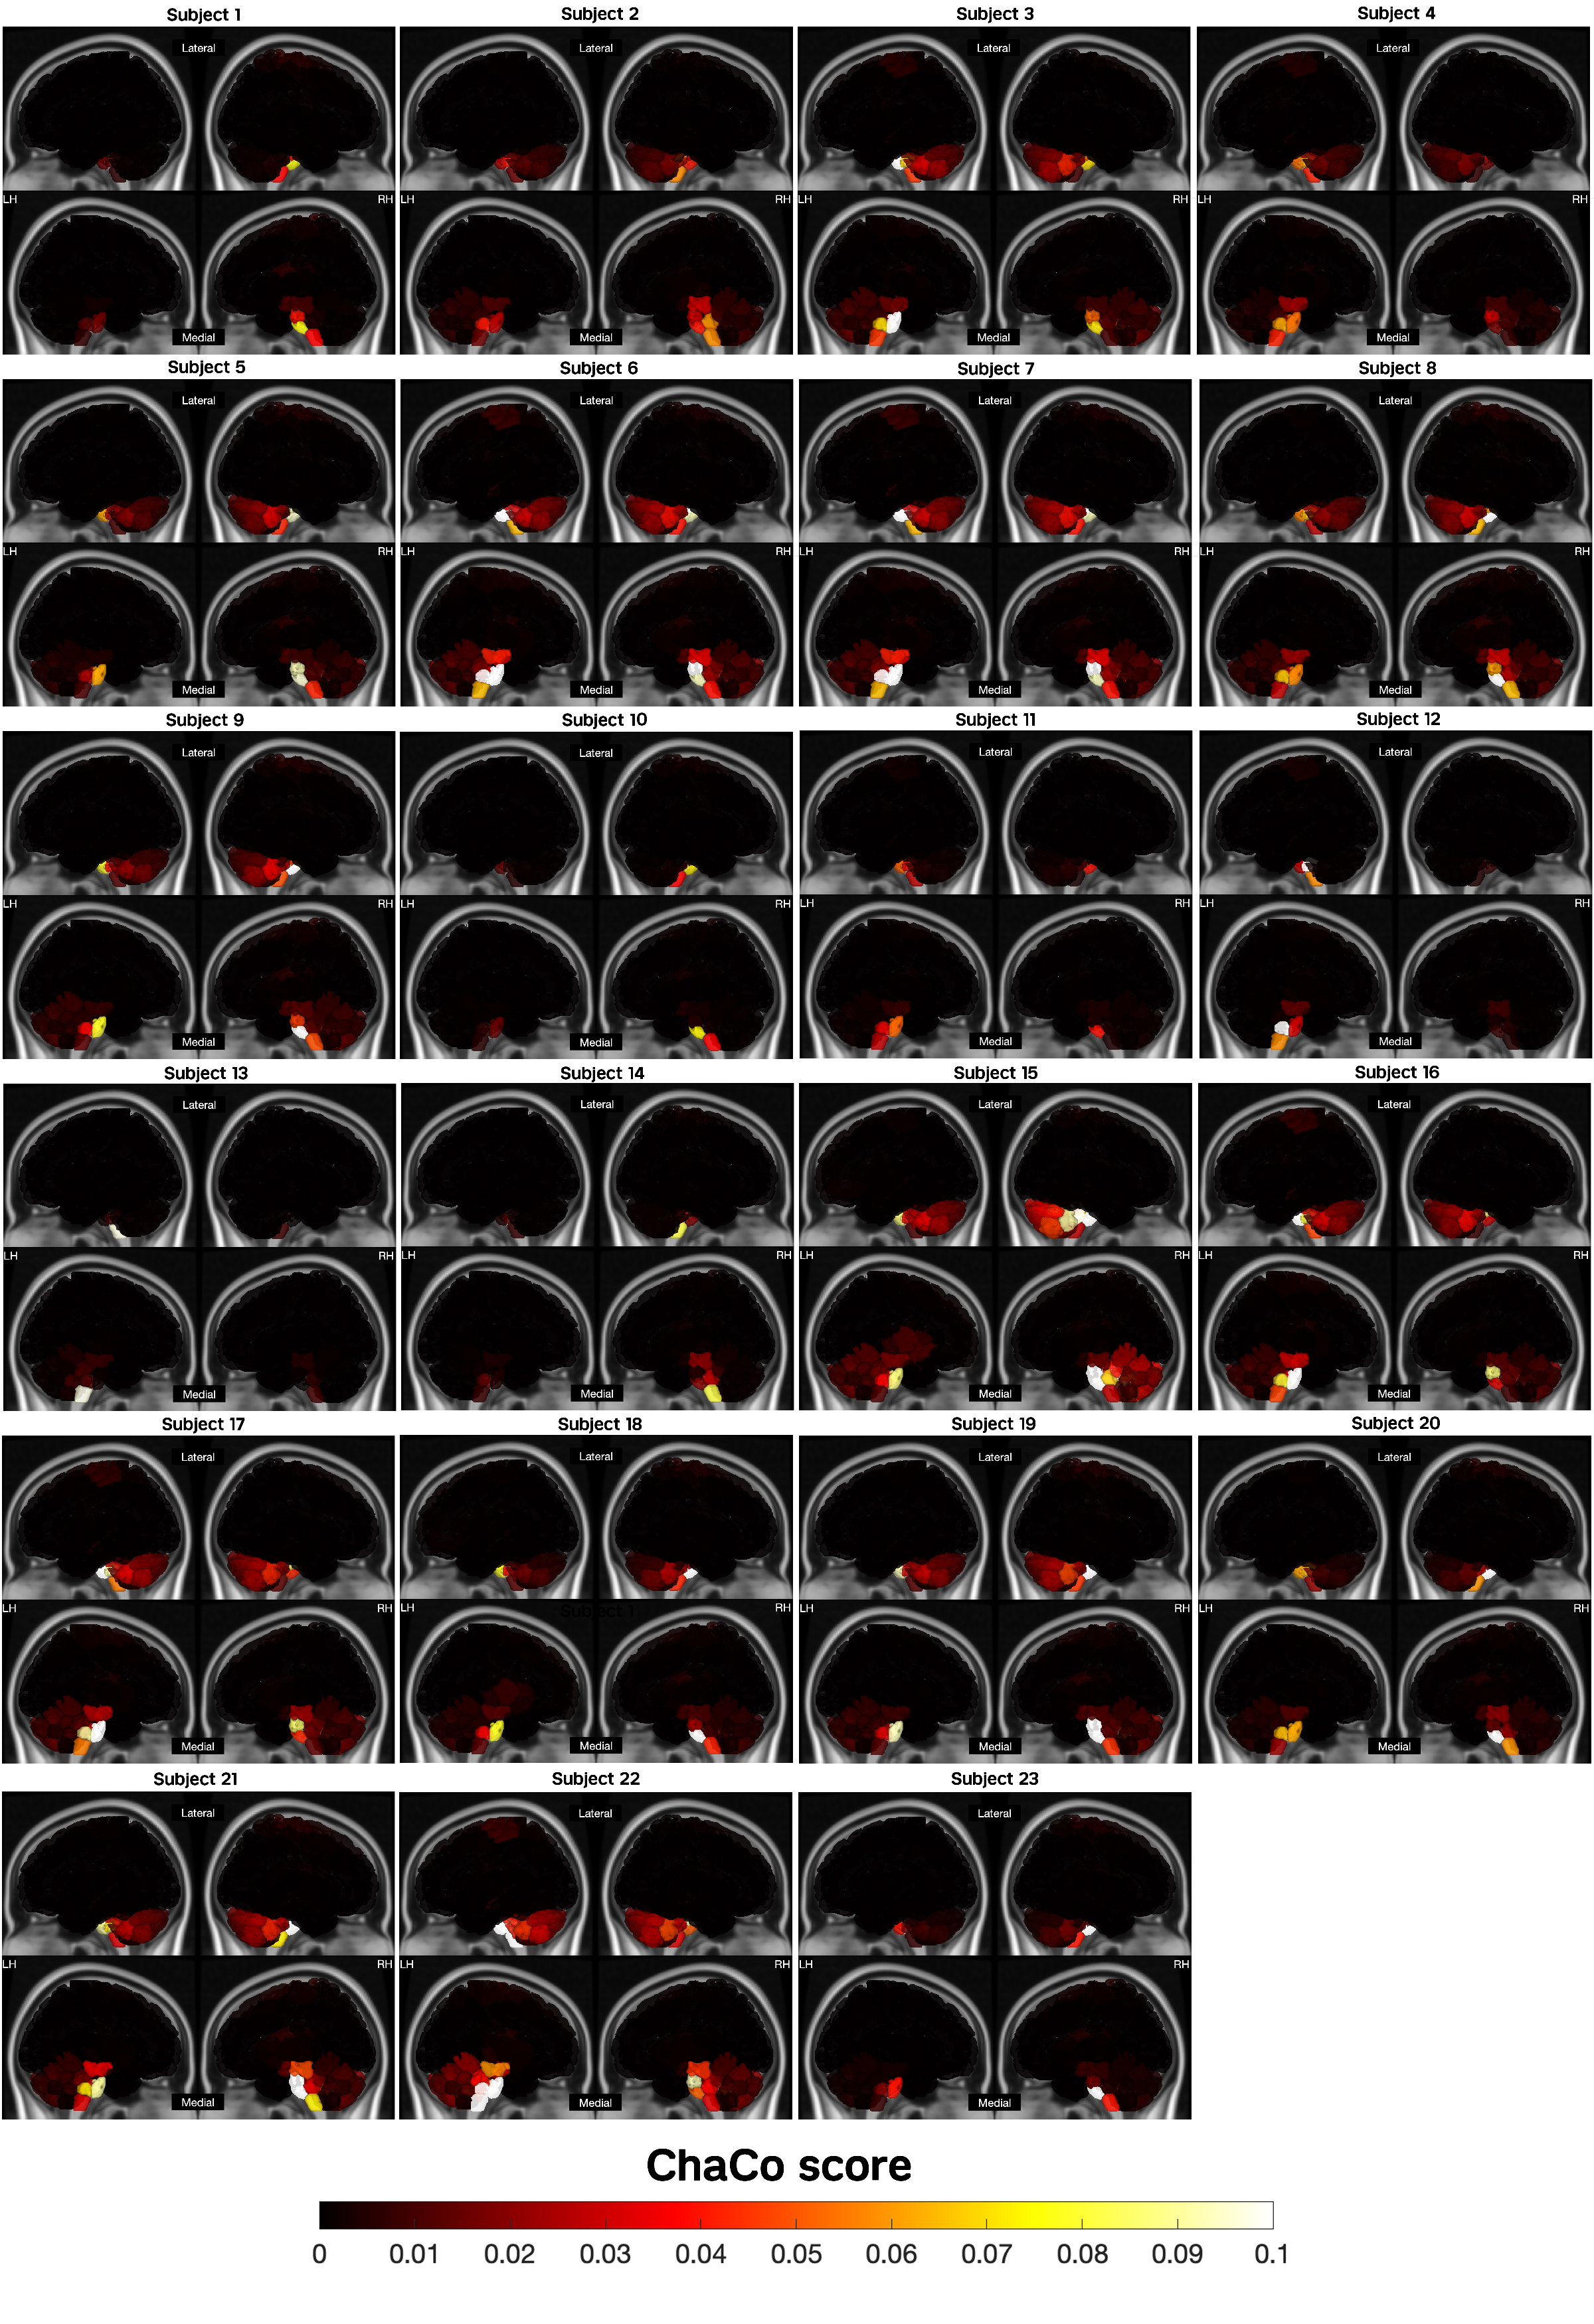
\includegraphics[width=0.9\textwidth]{allsubjects_chaco.pdf}
		\caption{Regional ChaCo scores of all subjects displayed on glass brains displaying the number of streamlines terminating in each region that intersect with the lesion, normalized for the total number of streamlines terminating in that region. Top row of each subject inset: lateral view, bottom row of each inset: medial view.}
		\label{chacoscores}
		\centering
\end{figure}

\begin{figure}[h] %	\label{chaco_remap_noremap}
	\includegraphics[width=0.9\textwidth]{chaco_remap_noremap.png}
	\caption{Paired t-tests determining whether there is a significant differene between the ChaCo scores of nodes that remap to different nodes versus those that do not. Remap patterns for the comparison between session 1 and 2 are shown; similar results are observed for other time points. No FDR correction}	\centering
	\label{chaco_remap_noremap}
\end{figure}
	
\begin{figure}[h] %  \label{remap_matrices}
		\begin{subfigure}{0.53\textwidth}
			\includegraphics[width=1\textwidth]{beta0/figures/remapping_matrices_S1S2.png}
			\caption{Remap matrix for S1-S2}
		\end{subfigure}
		\begin{subfigure}{0.53\textwidth}
			\includegraphics[width=1\textwidth]{beta0/figures/remapping_matrices_S2S3.png}
			\caption{Remap matrix for S2-S3}
		\end{subfigure}
		
		\vskip\baselineskip
		
		\begin{subfigure}{0.53\textwidth}
			\includegraphics[width=1\textwidth]{beta0/figures/remapping_matrices_S3S4.png}
			\caption{Remap matrix for S3-S4}
		\end{subfigure}
		\begin{subfigure}{0.53\textwidth}
			\includegraphics[width=1\textwidth]{beta0/figures/remapping_matrices_S4S5.png}
			\caption{Remap matrix for S4-S5}
		\end{subfigure}
    \caption{Permutation matrices across all 23 subjects.  Each row and column represents the number of subjects where that specific remapping (node $i$ = row $i$ to node $j$ = column $j$). The colorbar was cutoff at 7 subjects to improve visibility of off-diagonal elements.  }
    \label{remap_matrices}
\end{figure}
	
\begin{figure}[h] %\label{costmat}
    \includegraphics[width=0.9\textwidth]{costmat.png}
    	\caption{Cost matrix indicating the cost of remapping nodes from session 2 (vertical axis) to every other node in session 1 (horizontal axis).}
    \label{costmat}
\end{figure}
    
\begin{figure}[h] %\label{sumremaps_yeo}
		\includegraphics[width=1\textwidth]{sum_remaps_yeo.png}
		\caption{Sum of remaps within 8 functional networks; values in cells represent the total number of swaps between nodes in each network (only including off-diagonal remappings that occur within the same network; i.e. original and target nodes are in the same network) across subjects. }
		\centering
		\label{sumremaps_yeo}
\end{figure}

\begin{figure}[h]%cst lesion load + lesion vol vs remaps
		\begin{subfigure}[t]{.5\textwidth}
			\includegraphics[width=1\textwidth]{lesionvol_remapss1s2.png}
			\caption{Lesion volume in mm$^{3}$}
			\centering
			\label{vollesion}
		\end{subfigure}
		\begin{subfigure}[t]{.5\textwidth}
			\includegraphics[width=1\textwidth]{lesionload_remapss1s2.png}
			\caption{Lesion load on the CST calculated as the proportion of the CST that intersects with the binary lesion mask (calculated on the ipsilesional CST)}
			\centering
			\label{cstlesion}
		\end{subfigure}
	\caption{The extent of the lesion's impact on the ipsilesional corticospinal tract is associated with the number of remaps between session 1 and 2 whereas the total lesion volume is not.}
\end{figure}

\begin{figure}[h] %label{FD} vs remaps
		\includegraphics[width=0.9\textwidth]{diff_remaps_diff_FD.png}
		\caption{Correlation between difference in motion (as measured by framewise displacemetn) between 2 scans and the amount of remaps between the two scans.}	\centering
		\label{FD}
\end{figure}

% Regularization results
\begin{figure}[h] % beta vs total number of swaps
	\includegraphics[width=0.9\textwidth]{betareg.png}
	\caption{Proportion of swaps across all subjects and nodes with varying beta parameters. Circles in the top left figure indicate beta parameters chosen for subsequent analyses with varying $\beta$ parameters.}	\centering
	\label{betareg}
\end{figure}

\begin{figure}[h] %sum of remaps within each ofr hte 8 functional netowrks
	\includegraphics[width=1\textwidth]{beta_nswaps.png}
	\caption{Impact of $\beta$ on the sum of remaps within 8 functional networks, displayed separately depending on the source and target node's position relative to the lesion. (ipsilesional, same side as the lesion, and contralesional, opposite side as the lesion).  Ipsi = ipsilesional, contra = contralesional. Ipsi-ipsi = ipsilesional node mapping to another ipsilesional node. Ipsi-contra = ipsilesional node mapping to a contralesional node. Conta-contra = contralesional node mapping to another contralesional node. Contra-ipsi = contralesional node mapping to an ipsilesional node. }	\centering
	\label{beta_nswaps}
\end{figure}

\begin{figure}[h] %beta vs correlation between chaco and remaps
	\begin{subfigure}{.5\textwidth}
		\fbox{\includegraphics[width=1\textwidth]{beta0/figures/corr_remapping_chaco.png}}
		\caption{Beta 1 ($\beta $ = 0)}
		\centering

	\end{subfigure}
	\begin{subfigure}{.5\textwidth}
		\fbox{\includegraphics[width=1\textwidth]{beta1/figures/corr_remapping_chaco.png}}
		\caption{Beta 2 ($\beta $ = 1e-3)}
		\centering

	\end{subfigure}
     \vskip\baselineskip
	\begin{subfigure}{.5\textwidth}
		\fbox{\includegraphics[width=1\textwidth]{beta2/figures/corr_remapping_chaco.png}}
		\caption{Beta 3 ($\beta $ = 2e-3)}
		\centering

	\end{subfigure}
	\begin{subfigure}{.5\textwidth}
		\fbox{\includegraphics[width=1\textwidth]{beta3/figures/corr_remapping_chaco.png}}
		\caption{Beta 4 ($\beta $ = 3e-3)}
		\centering

	\end{subfigure}
	
	\caption{Varying betas - correlation between number of remaps and ChaCo scores}
	\label{betas_corrchaco}
\end{figure}

\begin{figure}[h] %betas - baselineFM vs remaps1s2
	\begin{subfigure}{.5\textwidth}
		\fbox{\includegraphics[width=1\textwidth]{beta0/figures/baselineFM_remaps_s1s2.png}}
		\caption{Beta 1 ($\beta$ = 0)}
		\centering
	\end{subfigure}
	\begin{subfigure}{.5\textwidth}
		\fbox{\includegraphics[width=1\textwidth]{beta1/figures/baselineFM_remaps_s1s2.png}}
		\caption{Beta 2 ($\beta$ = 1e-3)}
		\centering
	\end{subfigure}
     \vskip\baselineskip
	\begin{subfigure}{.5\textwidth}
		\fbox{\includegraphics[width=1\textwidth]{beta2/figures/baselineFM_remaps_s1s2.png}}
		\caption{Beta 3 ($\beta$ = 2e-3)}
		\centering
		
	\end{subfigure}
	\begin{subfigure}{.5\textwidth}
		\fbox{\includegraphics[width=1\textwidth]{beta3/figures/baselineFM_remaps_s1s2.png}}
		\caption{Beta 4 ($\beta$ = 3e-3)}
		\centering
		
	\end{subfigure}
	\caption{Varying beta does not change the significance of the relationship between total number of remaps between session 1 and session 2 and baseline Fugl-Meyer scores }
	\label{beta_recovery_remaps}
\end{figure}

\begin{figure}[h] % betas - delta FM n remaps
	\begin{subfigure}[t]{.45\textwidth}
		\fbox{\includegraphics[width=1\textwidth]{beta0/figures/remaps_recovery_sessionspecific.png}}
		\caption{Beta 1 ($\beta$ = 0)}

	\end{subfigure}
	\begin{subfigure}[t]{.45\textwidth}
		\fbox{\includegraphics[width=1\textwidth]{beta1/figures/remaps_recovery_sessionspecific.png}}
		\caption{Beta 2 ($\beta$ = 1e-3)} 
		\centering
	\end{subfigure}

     \vskip\baselineskip
     
	\begin{subfigure}[t]{.45\textwidth}
		\fbox{\includegraphics[width=1\textwidth]{beta2/figures/remaps_recovery_sessionspecific.png}}
		\caption{Beta 3 ($\beta$ = 2e-3)}
		\centering

	\end{subfigure}
	\begin{subfigure}[t]{.45\textwidth}
		\fbox{\includegraphics[width=1\textwidth]{beta3/figures/remaps_recovery_sessionspecific.png}}
		\caption{Beta 4 ($\beta$ = 3e-3)}

	\end{subfigure}
	\caption{Varying beta generally does not alter the relationships observed between session-specific increases in Fugl-Meyer scores and the number of remaps betwen sessions.}
	\label{beta_recovery_remaps_alllsess}
\end{figure}
	

\begin{figure}[h] % temporal signal-to-noise ratio: TSNR=MEAN/stdev(non-artifact thermal noise) 
	\includegraphics[width=1\textwidth]{HCP_SNR.png}
	\caption{Keith's SNR calculations on the test-retest HCP data: temporal signal-to-noise ratio: TSNR=MEAN/stdev(non-artifact thermal noise)}
	\label{HCP_SNR}
\end{figure}

	\clearpage
	\printbibliography


	
	
\end{document}
